\chapter{Algorithmes et\\programmation} \label{T15}

\newcommand{\fourmi}[3]{\rput{#3}(#1,#2){\psdot[linecolor=red,dotstyle=triangle*,linewidth=1mm](0,0)}}

\bigskip

\begin{figure}[h]
   \centering
      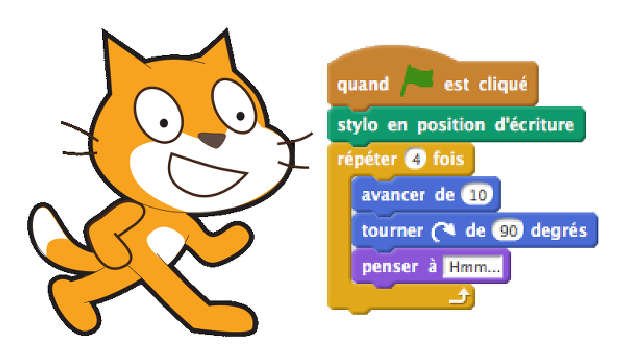
\includegraphics[height=5cm]{Transversal/Images/T15_intro_Scratch}
   \caption{Scratch}
\end{figure}

\begin{prerequis}[Un peu d'histoire]
   Le numérique fait maintenant partie intégrante des programmes de mathématiques. L'introduction dans les programmes de mathématiques à tous niveaux du codage et de l'algorithmique a transformé petit à petit l'utilisation de langages de programmation vers des logiciels utilisant des pseudo-langages et des langages visuels.
   Les premiers langages de programmation sont antérieurs aux ordinateurs modernes : dès 1801, les cartes perforées du {\it métier Jacquard} font figure d'algorithmes puisqu'elles permettent de générer les mouvements du métier à tisser de manière automatique. \\
   À l'école et au collège on utilise régulièrement le logiciel scratch, et d'autres applications qui y ressemblent : il s'agit de déplacer des blocs qui s'imbriquent en se suivant ou les uns dans les autres afin de former des programmes.
\end{prerequis}


%%%%%%%%%%%%%%%%%%%%%%%%%%%%%%%
%%%%%%%%%%%%%%%%%%%%%%%%%%%%%%%
\cours


%%%%%%%%%%%%%%%%%%
\section{Algorithmes et langages de programmation} %%%

\begin{definition}[Algorithme]
   Un {\bf algorithme} est une liste ordonnée et logique d'instructions permettant de réaliser une tâche de manière automatisée.
\end{definition}

\bigskip

   Généralement, un algorithme se compose en trois parties : les données de départ (entrées), la liste des instructions (traitement), le résultat (sortie).

\begin{exemple*1}
   Les recettes de cuisine sont des d'algorithmes. \\ [1mm]
   {\hautab{1.5}{
      \begin{Ltableau}{1.11\linewidth}{3}{C{2.6}|p{9cm}|C{2.45}}
         \hline
         Étape 1 : données & Étape 2 : instructions & Étape 3 : résultat \\
         \hline
         3 oeufs & 1 - mélanger les oeufs et le sucre & \\
         150 g de farine & 2 - ajouter le beurre fondu, puis la farine & on obtient un \\
         100 g de sucre & 3 - couper les bananes en morceaux et les ajouter au mélange & succulent \\
         125 g de beurre & 4 - aromatiser avec le rhum et la vanille & gâteau-banane !  \\
         4 bananes péi & 5 - verser le tout dans un moule à cake beurré et fariné & \\
         rhum et vanille & 6 - laisser cuire environ 30 mn au four thermostat 6 & \\
         \hline   
      \end{Ltableau}}
   }
   \ \\ [-6mm]
\end{exemple*1}


\bigskip

   Un algorithme peut-être traduit, grâce à un langage de programmation, en un programme exécutable par un ordinateur. Ce langage peut être un langage formel, un langage textuel, un langage visuel (il s'agit en fait d'un pseudo-code qui est traduit par un logiciel en langage compréhensible par l'ordinateur).

\medskip

\begin{exemple*1}
   Programmation d'un algorithme qui calcule $2(x-3)$ pour un réel $x$ donné. \\ [1mm]
   {\hautab{1.5}{
      \begin{Ltableau}{0.96\linewidth}{3}{p{4cm}|p{3cm}|p{5cm}}
         \hline
         Langage courant & Langage python 3 & Langage scratch \\
         \hline
         \begin{minipage}{4cm}
            Choisir un nombre $x$ \\
            lui soustraire 3 \\
            multiplier le résultat par 2 \\
            donner le résultat \\
         \end{minipage}
         & 
         \begin{minipage}{4cm}
            \texttt{x=input('x=')} \\
            \texttt{x=x-3} \\
            \texttt{x=2*x} \\
            \texttt{print(x)} \\
         \end{minipage}
         &
         \begin{minipage}{4cm}
         \vspace*{1mm}
         {\setscratch{scale=1}
            \begin{scratch}    
               \blockinit{quand \greenflag est cliqué}
               \blocksensing{demander \ovalnum{valeur de x} et attendre}
               \blockvariable{mettre \selectmenu{x} à \ovalsensing{réponse}}
               \blockvariable{mettre \selectmenu{x} à \ovaloperator{\ovaloperator{\ovalvariable{x} - \ovalnum{3}}}}
               \blockvariable{mettre \selectmenu{x} à \ovaloperator{\ovaloperator{2 * \ovalvariable{x}}}}
               \blocklook{dire \ovalvariable{x}}
            \end{scratch}
         }
         \vspace*{1mm}
         \end{minipage} \\
         \hline   
      \end{Ltableau}}
   }
   \ \\ [-6mm]
\end{exemple*1}

\bigskip    

Actuellement, les logiciels préconisés dans le secondaires sont Scratch au collège et Python (après des années d'Algobox) au lycée. Les sessions relativement récentes (à partir de 2015) du DNB et du CRPE ont vu apparaître de multiples exercices basés sur Scratch.

\bigskip


%%%%%%%%%%%%%%%%%%%%%%%%%
%%%%%%%%%%%%%%%%%%%%%%%%%
\section{Utilisation de Scratch}

   Scratch est \href{https://scratch.mit.edu/download}{\blue téléchargeable} gratuitement. Développé par le MIT, c'est un langage de programmation qui facilite la création d’histoires interactives, de dessins animés, de jeux, de simulations numériques\dots{} La version actuelle est la 3.0 qui offre une inetrface graphique légèrement différente à sa prédécesseur, la 2.0. \medskip

\hspace*{-8mm}
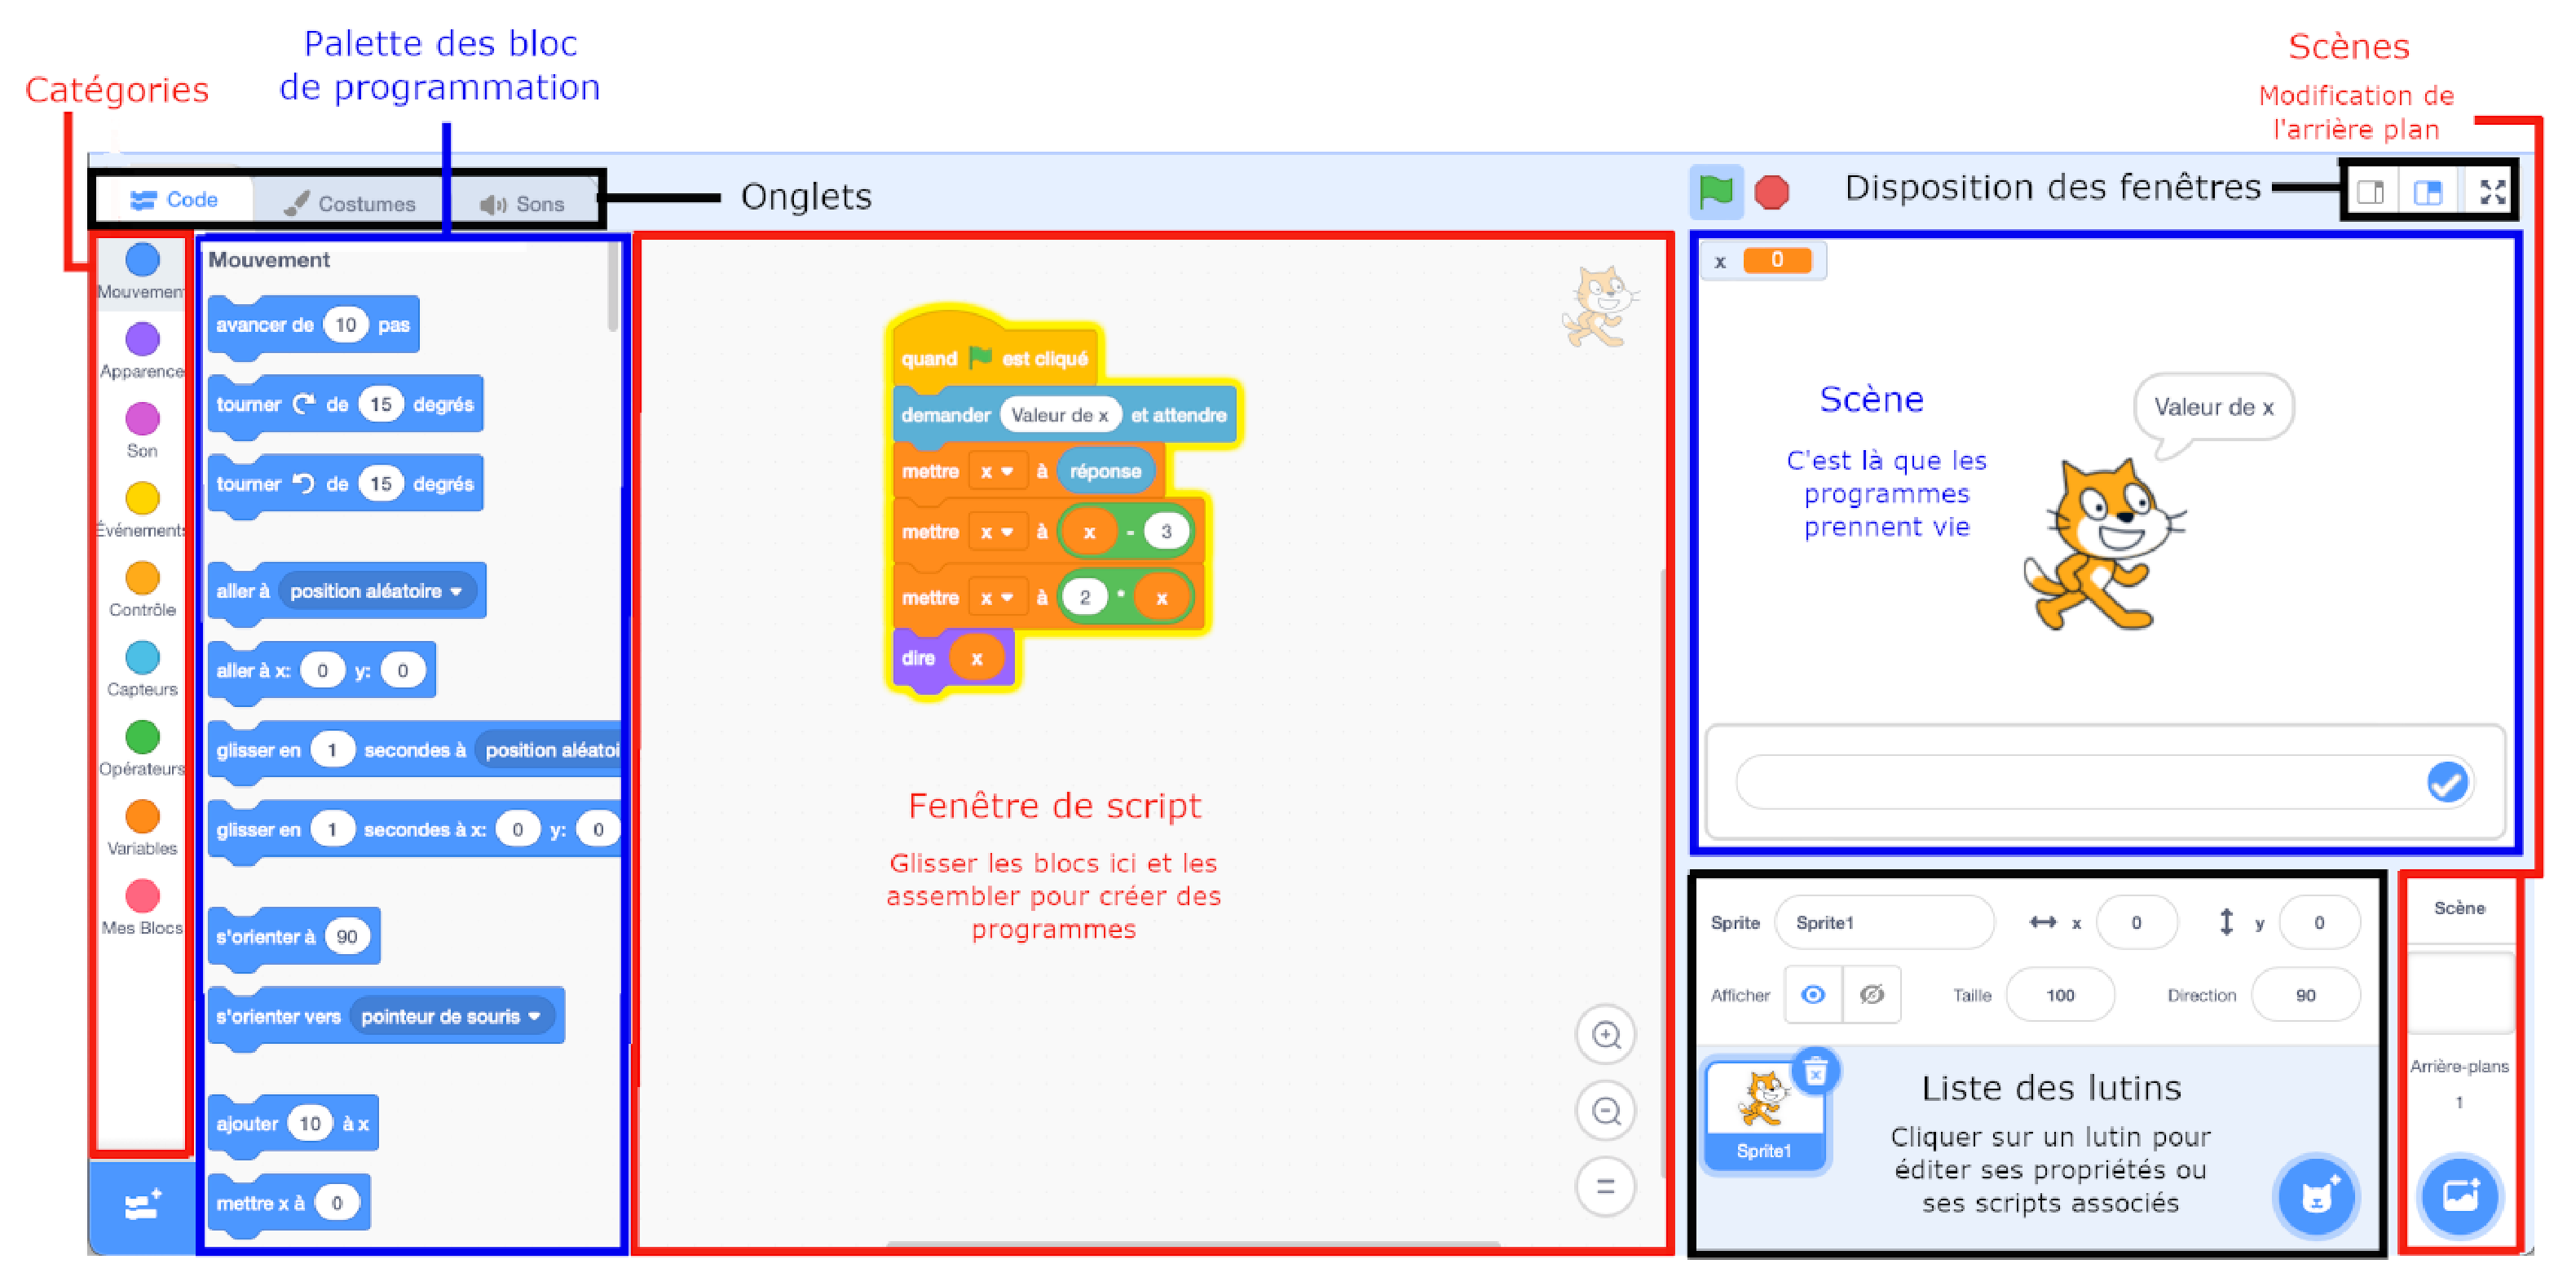
\includegraphics[width=18.5cm]{Transversal/Images/T15_cours_interface} 
\smallskip

   Tout le code est directement inscrit dans la langue choisie sous forme de blocs de couleur permettant d'exécuter une action précise. Il existe plusieurs catégories de blocs : \\ [2mm]
   {\hautab{1.5}{
   \begin{tabular}{C{0.5}p{3.5cm}p{12cm}}
      \pscircle[fillstyle=solid,fillcolor=blue!60](0,0.15){0.3}
      &
      Blocs de mouvement
      &
      Permettent de déplacer et positionner les lutins. \\
      \pscircle[fillstyle=solid,fillcolor=blue!30](0,0.15){0.3}
      &
      Bloc d'apparence
      &
      Servent à modifier l'apparence des lutins. \\
      \pscircle[fillstyle=solid,fillcolor=violet!80](0,0.15){0.3}
      &
      Blocs de son
      &
      Permettent de jouer des sons. \\
      \pscircle[fillstyle=solid,fillcolor=yellow](0,0.15){0.3}
      &
      Blocs d'événements
      &
      Permettent de lancer des scripts ou déclencher des événements. \\
      \pscircle[fillstyle=solid,fillcolor=orange!60](0,0.15){0.3}
      &
      Blocs de contrôle
      &
      Servent à contrôler l'exécution du script (pause, conditions, répétitions, arrêt). \\
      \pscircle[fillstyle=solid,fillcolor=cyan!50](0,0.15){0.3}
      &
      Capteurs
      &
      Servent à mesurer ou détecter certaines valeurs et à poser des questions. \\
      \pscircle[fillstyle=solid,fillcolor=green](0,0.15){0.3}
      &
      Blocs d'opérateurs
      &
      Servent à effectuer des opérations et à manipuler les chaînes de caractères. \\
      \pscircle[fillstyle=solid,fillcolor=orange](0,0.15){0.3}
      &
      Blocs de données
      &
      Permettent de stocker des informations en mémoire. \\
      \pscircle[fillstyle=solid,fillcolor=magenta!80](0,0.15){0.3}
      &
      Blocs personnels
      &
      Création de blocs personnels permettant de répéter certaines actions. \\
   \end{tabular}}
   }

\smallskip

Dans scratch 3.0, il est également possible d'ajouter des extensions comme le stylo ou des extensions pour programmer des robots éducatifs. \\
Au lieu d’écrire du texte, on manipule des blocs que l'on assemble de manière logique et ordonnée en suivant un algorithme. 

Pour qu'un programme puisse démarrer, il faut un bloc de départ événementiel, qui peut être activé en cliquant sur le drapeau vert ou en pressant sur une touche : \begin{scratch}
   {\setscratch{scale=0.75}
      \blockinit{quand \greenflag est cliqué}
   }
\end{scratch}
\; ou \;
\begin{scratch}
   \blockinit{Quand \selectmenu{espace} est cliqué}
\end{scratch}

\bigskip

{\bf Une boucle} permet d'itérer une séquence indéfiniment ou un certain nombre de fois. \\ [-8mm]
\begin{exemple}
   \vspace*{1mm}
   {\setscratch{scale=0.8}
   \begin{scratch}
      \blockpen{stylo en position d’écriture}
      \blockrepeat{répéter \ovalnum{4} fois}
         {
         \blockmove{avancer de \ovalnum{10}}
         \blockmove{tourner \turnright{} de \ovalnum{90} degrés}
         }
   \end{scratch}
   }
   \correction
      Ce script propose d'utiliser le lutin \og stylo \fg{} pour dessiner un carré de côté 10 pixels. \\
      La boucle crée un segment de longueur 10 pixels puis fait tourner la direction d'écriture du crayon de \udeg{90} dans le sens horaire (ou sens indirect). \\
      Cette boucle, itérée 4 fois, trace le carré.
\end{exemple}

\bigskip

{\bf Une instruction conditionnelle} (si et si-sinon) permet d’engager une action suivant qu’une condition est réalisée ou non. \\ [-8mm]
\begin{exemple}
   \vspace*{1mm}
   {\setscratch{scale=0.8}
   \begin{scratch}
      \blocksensing{demander \ovalnum{6 x 7 = ?} et attendre}
      \blockifelse{si \ovaloperator{\ovalsensing{réponse} = \ovalnum{42} alors}}
         {\blocklook{dire \ovalnum{C'est juste} pendant \ovalnum{2} secondes}}
         {\blocklook{dire \ovalnum{C'est faux} pendant \ovalnum{2} secondes}}
   \end{scratch}
   }
   \correction
      Le bloc de capteur demande le résultat de $6\times7$ et met en mémoire la réponse dans le bloc \og réponse \fg. \\
      Si la réponse est 42, alors le programme écrit que \og c'est juste \fg{} pendant 2 secondes, et sinon (donc si la réponse est fausse), il dit que \og c'est faux \fg.
\end{exemple}

\bigskip

{\bf Une variable} est un nom donné à un emplacement en mémoire contenant une information. \\ [-8mm]  
\begin{exemple}   
   {\vspace*{1mm}
   \setscratch{scale=0.8}
   \begin{scratch}    
      \blocksensing{demander \ovalnum{valeur de x} et attendre}
      \blockvariable{mettre \selectmenu{x} à \ovalsensing{réponse}}
      \blockvariable{mettre \selectmenu{x} à \ovaloperator{\ovaloperator{\ovalvariable{x} * \ovalvariable{x}}}}
      \blocklook{dire \ovalnum{Le carré de x vaut :} \ovalvariable{x}}
   \end{scratch}
   }
   \correction
      Une variable $x$ a été crée. \\
      On affecte la valeur demandée par le bloc capteur (stocké dans \og réponse \fg) à la variable $x$. \\
      Ensuite, on affecte la valeur de $x\times x$, c'est-à-dire $x^2$ à la variable $x$. \\
      Le carré du nombre demandé est alors affiché.
\end{exemple}

\bigskip

{\bf Un bloc personnalisé} permet de définir un programme annexe à utiliser dans le programme principal par exemple. \\ [-8mm]
\begin{exemple}[0.5]   
   {\setscratch{scale=0.8}
   \begin{scratch}
      \initmoreblocks{définir \namemoreblocks{trace carré}}
      \blockrepeat{répéter \ovalnum4 fois}
         {
         \blockmove{avancer de \ovalnum{10}}
         \blockmove{tourner \turnright{} de \ovalnum{90} degrés}
         }
     \end{scratch}
     \quad
     \begin{scratch}
        \blockinit{Quand \greenflag est cliqué}
        \blockpen{stylo en position d’écriture}
        \blockrepeat{répéter \ovalnum{10} fois}
           {
           \blockmoreblocks{trace carré}
           \blockmove{avancer de \ovalnum{20}}
           }
      \end{scratch}
      }
   \correction
      Le premier script propose de définir un carré de côté 10 pixels comme dans le premier exemple. C'est un programme annexe. \\
      Dans le second script, la boucle de répétition trace un carré de côté 10 pixels, puis avance de 20 pixels. \\
      Cette boucle, répétée 10 fois, trace donc 10 carrés de côté 10 pixels sur une même ligne, séparés entre eux de 10 pixels.
\end{exemple}


%%%%%%%%%%%%%%%%%%%%%%%%%%%%%%%%
%%%%%%%%%%%%%%%%%%%%%%%%%%%%%%%%
\activites

\begin{activite}[Groupement 1 - Exercice 4 : Scratch et géométrie]
   \ \\ [-16mm]
   \begin{QCM}
      \begin{minipage}{10cm}
         Le programme ci-contre ({\it programme 1}) a été écrit avec le logiciel Scratch.
            \begin{enumerate}
               \item En prenant $C = 50$ et 1 cm pour 10 pixels, tracer la figure construite en utilisant le {\it programme 1}. 
              \item Quelle est la nature de la figure tracée ? Justifier la réponse.     
               \item On écrit le {\it programme 2} en utilisant le bloc précédent, afin d’obtenir la figure représentée ci-après.
                  \begin{center}
                  {\psset{unit=0.35}
                     \begin{pspicture}(-20,-1)(6,16)
                        \pspolygon(0,0)(3,0)(5.12,2.12)(3;45)
                        \rput{45}(0,0){\pspolygon(0,0)(6,0)(10.24,4.24)(6;45)}
                        \rput{90}(0,0){\pspolygon(0,0)(9,0)(15.36,6.36)(9;45)}
                        \rput{135}(0,0){\pspolygon(0,0)(12,0)(20.49,8.49)(12;45)}
                     \end{pspicture}} \\ [2mm]
                     Rappel : \begin{scratch}
                        \blockmove{s’orienter à \ovalnum{90}}
                     \end{scratch} \\
                     \hspace*{26mm}
\includegraphics[width=15mm]{Transversal/Images/T15_ex_orienter}
                  \end{center}
                  \begin{enumerate}
                     \item Quelles valeurs attribuer aux lettres $A$ et $N$ dans le programme 2 pour obtenir la figure correspondante ?   
                     \item Quelle est la valeur de la variable $C$ une fois le programme exécuté ? \\ [-10mm]
                  \end{enumerate}
               \item Comment peut-on modifier le programme 2 pour obtenir la figure ci-contre pour laquelle chaque segment mesure 30 pixels ?
                  \begin{center}
                  {\psset{unit=0.3}
                     \begin{pspicture}(-8,-10.5)(8.5,9)
                        \pspolygon(0,0)(5,0)(8.53,3.53)(5;45)
                        \rput{90}(0,0){\pspolygon(0,0)(5,0)(8.53,3.53)(5;45)}
                        \rput{180}(0,0){\pspolygon(0,0)(5,0)(8.53,3.53)(5;45)}
                        \rput{270}(0,0){\pspolygon(0,0)(5,0)(8.53,3.53)(5;45)}
                     \end{pspicture}}
                  \end{center}
            \end{enumerate}
      \end{minipage}
      \hfill
      \begin{minipage}{5cm}
         {\it Programme 1} \\
         \begin{scratch}
            \initmoreblocks{définir \namemoreblocks{motif}}
            \blockrepeat{répéter \ovalnum2 fois}
               {\blockmove{avancer de \ovalvariable{C} pas}
                \blockmove{tourner \turnleft{} de \ovalnum{45} degrés}
                \blockmove{avancer de \ovalvariable{C} pas}
                \blockmove{tourner \turnleft{} de \ovalnum{135} degrés}
               }
         \end{scratch} \\ [10mm]
         {\it Programme 2} \\
         \begin{scratch}   
            \blockinit{Quand \greenflag est cliqué}
           \blockmove{aller à x: \ovalnum0 y: \ovalnum0}
            \blockmove{s’orienter à \ovalnum{90}}
            \blockpen{effacer tout}
            \blockpen{stylo en position d’écriture}
            \blockvariable{mettre \selectmenu{C} à \ovalnum{30}}
            \blockrepeat{répéter \ovalvariable{N} fois}
               {\blockmoreblocks{motif}
                \blockmove{tourner \turnleft{} de \ovalvariable{A} degrés}
                \blockvariable{ajouter \ovalnum{30} à \selectmenu{C}}
               }
         \end{scratch}
         \vfill
      \end{minipage}
   \end{QCM}
   
   \bigskip
   
   \textcolor{G1}{
   {\bf Exemple de corrigé.} \smallskip
      \begin{enumerate}
         \item On obtient le dessin suivant : \\
            \begin{pspicture}(-1,-0.5)(8.5,4.5)
               \small
               \psset{linecolor=G1}
               \pspolygon(0,0)(5,0)(8.53,3.53)(5;45)
               \rput(2.5,-0.3){5 cm}
               \rput{45}(7,1.5){5 cm}
               \psline[linestyle=dashed](5,0)(6,0)
               \psarc{->}(5,0){0.7}{0}{45}
               \rput(6,0.3){45°}
               \psline[linestyle=dashed](8.53,3.53)(9.24,4.24)
               \psarc{->}(8.53,3.53){0.6}{45}{180}
               \rput(8.3,4.5){135°}
            \end{pspicture}
         \item La première répétition fait tracer deux segments consécutifs. À la fin de la boucle, la rotation vers la gauche de 135° implique un angle de 45° $+$ 135° $=$ 180° entre le premier et le troisième segment. Ils sont donc parallèles. \\
            Le dernier segment, après une rotation de 45°, est parallèle au deuxième puisqu'ils forment un angle de \newline
            135° $+$ 45° $=$ 180°. \\
            On a donc un quadrilatère ayant ses côtés opposés parallèles deux à deux, c'est un parallélogramme. \\
            De plus, les quatre côtés sont de même mesure (50 pixels), \uline{c'est un losange de côté 50 pixels}.
         \item
            \begin{enumerate}
               \item $A$ correspond à l'angle de rotation du motif dans le sens inverse des aiguilles d'une montre, il est ici de 45° et $N$ correspond au nombre de répétitions du motif, c'est-à-dire 4. \\
                  \uline{On peut choisir $A =45$ et $n =4$ pour obtenir la figure donnée}.
               \item $C$ vaut initialement 30, et il est augmenté de 30 à chaque fin de répétition. En fin de programme, \uline{ il vaut donc $30+4\times30 =150$} (cependant, le côté du dernier losange tracé vaut 120).
            \end{enumerate}
         \item \uline{Il suffirait de donner la valeur de 90 à $A$ et de supprimer la ligne \og ajouter 30 à $C$ \fg}. \\
      \end{enumerate}}
\end{activite}

\vfill
\pagebreak


%%%%%%%%%%%%%%%%%%%%%%%%%%%%%%%
%%%%%%%%%%%%%%%%%%%%%%%%%%%%%%%
\begin{activite}[Groupement 2 - Exercice 4 - Question 1 : Scratch et calculs]
   \ \\ [-16mm]
   \begin{QCM}
      \begin{minipage}{8cm}
      Adam a réalisé le programme ci-contre à l’aide du logiciel Scratch.
         \begin{enumerate}
            \item Montrer que si le nombre de départ est 3, le résultat est égal à 9.
            \item Quel est le résultat donné par le programme si le nombre de départ est 2,4 ?
            \item Soit $x$ le nombre de départ. Montrer que le programme d’Adam retourne le nombre $2x^2-x-6$.           
         \end{enumerate}
      \end{minipage}
      \hfill
      \begin{minipage}{8cm}
         \begin{scratch}
            \blockinit{Quand \greenflag est cliqué}
            \blocksensing{demander \ovalnum{Choisir un nombre} et attendre}
            \blockvariable{mettre \selectmenu{nombre départ} à \ovalsensing{réponse}}
            \blockvariable{mettre \selectmenu{valeur 1} à \ovaloperator{\ovalnum{2} * \ovalvariable{nombre départ}}}
            \blockvariable{mettre \selectmenu{valeur 2} à \ovaloperator{\ovalvariable{valeur 1} + \ovalnum{3}}}
            \blockvariable{mettre \selectmenu{valeur 3} à \ovaloperator{\ovalvariable{nombre départ} - \ovalnum{2}}}
            \blockvariable{mettre \selectmenu{résultat} à \ovaloperator{\ovalvariable{valeur 2} * \ovalvariable{valeur 3}}}
            \blocklook{dire \ovaloperator{regrouper \ovalnum{Le résultat du programme est } et \ovalvariable{résultat}}}
         \end{scratch} \\ [7mm]
      \end{minipage}
   \end{QCM}
   
   \bigskip
   
   \textcolor{G1}{
   {\bf Exemple de corrigé.} \smallskip
      \begin{enumerate}
         \item On obtient les valeurs suivantes : \\
               nombre départ $\leftarrow 3$ \\
               valeur 1 $\leftarrow2\times3 =6$ \\
               valeur 2 $\leftarrow6+3 =9$ \\
               valeur 3 $\leftarrow3-2 =1$ \\
               résultat $\leftarrow9\times1 =9$ \\
               \uline{Si le nombre de départ est 3, alors le résultat est 9}.
         \item On obtient les valeurs suivantes : \\
               nombre départ $\leftarrow 2,4$ \\
               valeur 1 $\leftarrow2\times2,4 =4,8$ \\
               valeur 2 $\leftarrow4,8+3 =7,8$ \\
               valeur 3 $\leftarrow2,4-2 =0,4$ \\
               résultat $\leftarrow7,8\times0,4 =3,12$ \\
               \uline{Si le nombre de départ est 2,4, alors le résultat est 3,12}.
         \item On obtient les valeurs suivantes : \\
               nombre départ $\leftarrow x$ \\
               valeur 1 $\leftarrow2\times x =2x$ \\
               valeur 2 $\leftarrow2x+3$ \\
               valeur 3 $\leftarrow x-2$ \\
               résultat $\leftarrow(2x+3)\times(x-2)$ \\
               \uline{Si le nombre de départ est $x$, alors le résultat est $(2x+3)(x-2)$}.
      \end{enumerate}}
\end{activite}

\pagebreak


%%%%%%%%%%%%%%%%%%%%%%%%%%%%%%%
%%%%%%%%%%%%%%%%%%%%%%%%%%%%%%%
\begin{activite}[Groupement 3 - Exercice 4 : Scratch et géométrie]
   \ \\ [-16mm]
   \begin{QCM}
      Voici un programme écrit avec le logiciel Scratch. \\
      \begin{minipage}{5cm}
         \begin{scratch}[num blocks =true]
            \blockinit{Quand \greenflag est cliqué}
            \blockpen{effacer tout}
            \blockmove{aller à x: \ovalnum0 y: \ovalnum0}
            \blockmove{s’orienter à \ovalnum{90}}
            \blockrepeat{répéter \ovalnum{4} fois}
               {\blockpen{stylo en position d’écriture}
                \blockmove{avancer de \ovalnum{10} pas}
                \blockpen{relever le stylo}
                \blockmove{avancer de \ovalnum{10} pas}
                \blockmove{tourner \turnright{} de \ovalnum{90} degrés}
               }
         \end{scratch} \\ [7mm]
      \end{minipage}
      \qquad
      \begin{minipage}{10cm}
         \begin{enumerate}
            \item Représenter la figure obtenue lorsque le programme est exécuté. On prendra 1 mm pour 1 pixel (correspondant à 1 pas).     
            \item Marie souhaite obtenir la figure ci-dessous où chaque tiret mesure 10 pixels et est séparé du précédent de 10 pixels. Quelle(s) modification(s) doit-elle apporter au programme ?
               \begin{center}
                  \begin{pspicture}(0,-0.25)(7.5,0.5)
                     \multido{\n=0+1,\r=0.5+1.0}{8}{\psline(\n,0)(\r,0)}
                  \end{pspicture}
               \end{center}
            \item
               \begin{enumerate}
                  \item Léo souhaite modifier le programme donné pour que l’on obtienne la figure ci-dessous. \\
                     Quelle(s) modification(s) doit-il apporter au programme de départ ?
                     \begin{center}
                        \begin{pspicture}(-1.5,-1.5)(1.5,1.5)
                           \multido{\n=90+-45,\i=0+-45}{8}{\rput{\i}(1.21;\n){\psline(-0.5,0)(0,0)}}
                        \end{pspicture}
                     \end{center}          
                  \item Quel type de transformation géométrique permet de passer d’un tiret à un autre ?
               \end{enumerate}
         \end{enumerate}
      \end{minipage}
   \end{QCM}
   
   \bigskip
   
   \textcolor{G1}{
   {\bf Exemple de corrigé.} \smallskip
      \begin{enumerate}
         \item On obtient la figure suivante :
            \begin{center}
               \begin{pspicture}(0,-1.5)(1,1)
                  \multido{\n=90+-90,\i=0+-90}{9}{\rput{\i}(1;\n){\psline[linecolor=G1](-1,0)(0,0)}}
               \end{pspicture}
            \end{center}
         \item Il y a 8 tirets, donc il faut 8 répétitions, et les tirets sont alignés, ce qui signifie qu'il n'y a pas de rotation. \\
            Par conséquent, \uline{en ligne 5, il fait \og répéter 8 fois \fg{} et supprimer le ligne 10}.
         \item
            \begin{enumerate}
               \item Il y a 8 tirets, donc il faut 8 répétitions, et la rotation à droite est de 45°. \\
                  \uline{En ligne 5, on remplace 4 par 8 et en ligne 10, il faut changer 90 en 45}.
               \item \uline{On passe d'un tiret à l'autre par rotation de centre le centre de la figure et d'angle 45°}.
            \end{enumerate}
      \end{enumerate}}
\end{activite}


%%%%%%%%%%%%%%%%%%%%%%%%%%%%%%%%
%%%%%%%%%%%%%%%%%%%%%%%%%%%%%%%%
\exercicesbase


\begin{center}
   {\cursive Maîtriser les bases avec} \href{http://mathenpoche.sesamath.net}{
\includegraphics[width=3cm]{Nombres_et_calculs/Images/mathenpoche}} \\
   \bigskip
   {\hautab{0.85}
   \cursive
   \begin{Ltableau}{0.775\linewidth}{4}{C{1}|C{1}|p{7cm}|p{2.3cm}}
      \hline
      Classe & \texttt{N\degre} & Thème & Dans le cours \\
      \hline
      \textcolor{orange}{\bf 6\up{e}} & \texttt{A1} & Algorithme et programmation & 1. et 2. \\
      \hline
      \textcolor{cyan}{\bf 5\up{e}} & \texttt{A1} & Algorithme et programmation & 1. et 2. \\
      \hline
      \textcolor{violet}{\bf 4\up{e}} & \texttt{A1} & Algorithme et programmation & 1. et 2. \\
      \hline
      \textcolor{green}{\bf 3\up{e}} & \texttt{A1$\to$A8} & Algorithme et programmation & 1. et 2. \\
      \hline
   \end{Ltableau}}
\end{center}

\bigskip


\begin{exercice}[CRPE 2018 G2] %%%8
   Le programme ci-dessous a été écrit avec le logiciel Scratch pour faire se déplacer le lutin \og hélicoptère \fg{} de la case \og Nantes \fg{} à la case \og Paris \fg{} sur l’arrière-plan ci-dessOus, c’est-à-dire pour \og avancer \fg{} de deux cases et \og monter \fg{} d’une case.
   \begin{center}
      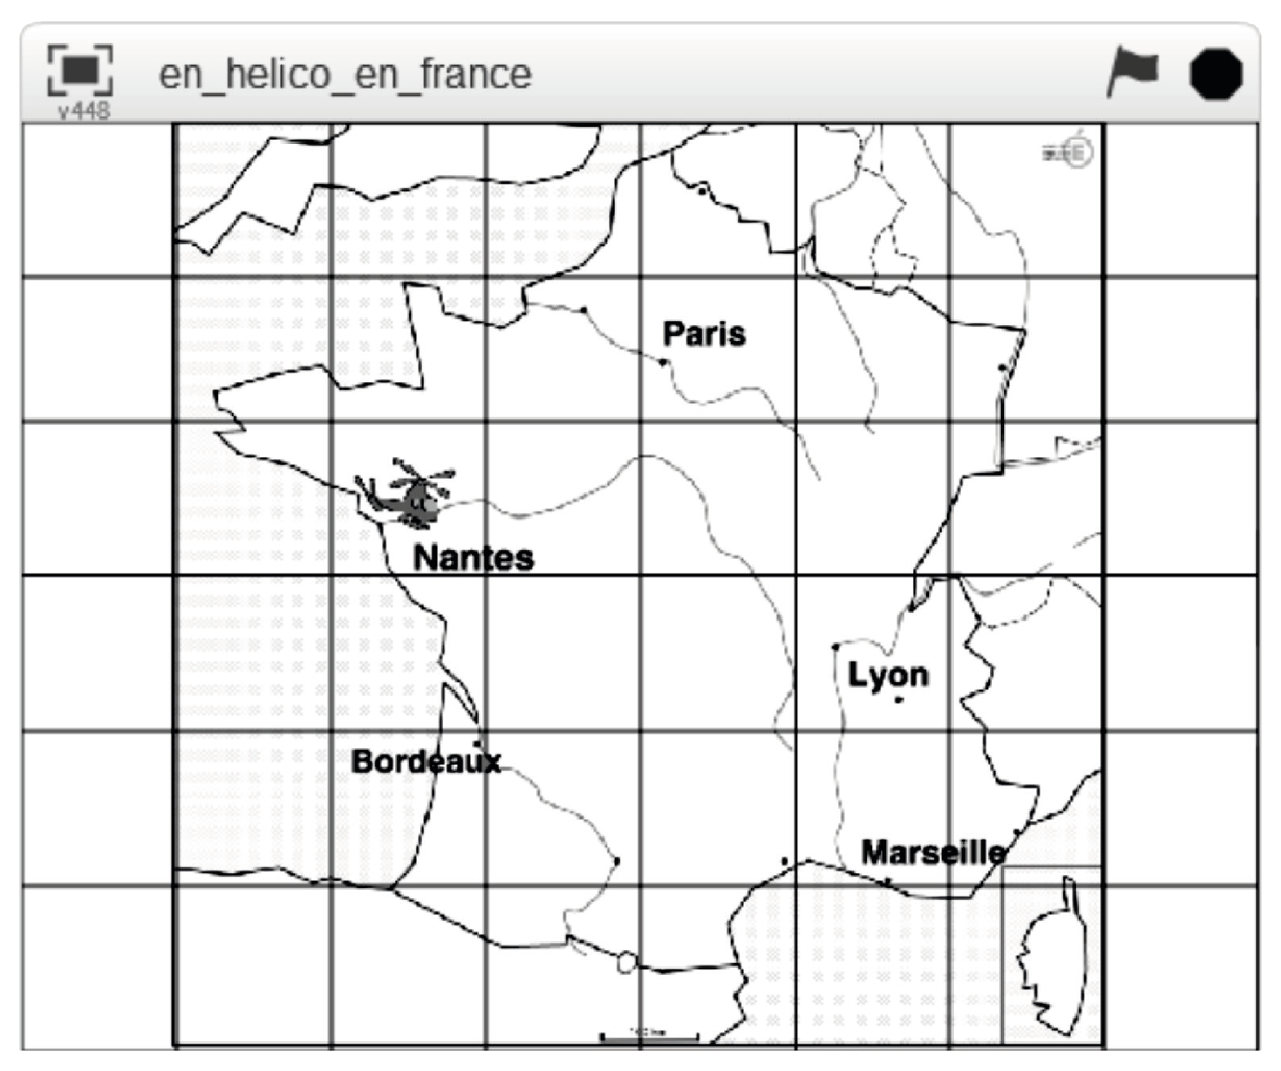
\includegraphics[width=10cm]{Transversal/Images/T15_ex_carte}
   \end{center}
   Un élève souhaite modifier le programme pour que l’hélicoptère se déplace de la case \og Nantes \fg{} à la case \og Lyon \fg{}. Par quels nombres doit-il remplacer les nombres \og 120 \fg{}, \og 270 \fg{} et \og 60 \fg{} ? Justifier votre réponse.
   \begin{center}
      \begin{scratch}
         \blockinit{Quand \greenflag est cliqué}
         \blockmoreblocks{Position initiale Nantes}
         \blockmoreblocks{se tourner vers l'est}
         \blockmove{avancer de \ovalnum{120} pas}
         \blockmove{tourner \turnright{} de \ovalnum{270} degrés}
         \blockmove{avancer de \ovalnum{60} pas}
      \end{scratch}
      \qquad
      \begin{scratch}
         \initmoreblocks{définir \namemoreblocks{Position initiale Nantes}}
         \blockmove{aller à x: \ovalnum{-93} y: \ovalnum{30}}
      \end{scratch}
      \qquad
      \begin{scratch}
         \initmoreblocks{définir \namemoreblocks{se tourner vers l'est}}
         \blockmove{s'orienter à \ovalnum{90}}
      \end{scratch}
   \end{center}
\end{exercice}

\begin{corrige}
   Pour aller de Nantes à Paris, l'hélicoptère se déplace vers l'est de 120 ce qui correspond à deux cases, donc une case correspond à un déplacement de 60. \\
   De la même manière, un déplacement vers le nord d'un case correspond à 60, les cases sont donc carrées. Donc, pour aller de Nantes à Lyon :
   \begin{itemize}
      \item il faut tout d'abord se déplacer de trois cases vers l'est, soit $3\times60 =180$ ;
      \item  puis il faut s'orienter vers de sud, donc tourner à droite d'un angle de \udeg{90} ;
      \item enfin, il faut se déplacer vers le sud d'une case, soit de 60.
   \end{itemize}
   Pour aller de Nantes à Lyon, {\blue il faut remplacer les nombres 120, 270 et 60 par 180, 90 et 60}.
\end{corrige}

\bigskip


\begin{exercice}[DNB 3017]
   L'image suivante représente la position obtenue au déclenchement du bloc \og Départ \fg{} d'un programme. \\
   L'arrière-plan est constitué de points espacés de 40 unités. Le chat a pour coordonnées $(-120\,;\,-80)$. \\
   Le but du jeu est de positionner le chat sur la balle représentée par le petit disque.
   \begin{center}
   {\psset{unit=0.7}
   \begin{pspicture}(-6,-3.3)(6,4.3)
      \multido{\n=-6+1}{13}{
      \multido{\na=-4+1}{9}{\psdots[dotscale=0.5](\n,\na)}}
      \psaxes[Dx=10,Dy=10]{->}(0,0)(-6,-4)(6,4)
      \uput[dl](0,0){O}
      \psdots[dotscale=2](4,3)
      \rput(-3,-2){Chat}
   \end{pspicture}}
   \end{center}
   \begin{enumerate}
      \item Quelles sont les coordonnées du centre de la balle représentée dans cette position?
      \item Dans cette question, le chat est dans la position obtenue au déclenchement du bloc départ. \\
      Voici le script du lutin \og chat \fg{} qui se déplace. \\
      \begin{minipage}{9cm}
         \begin{scratch}
            \blockinit{Quand \greenflag est cliqué}
            \blockmoreblocks{Départ}
         \end{scratch} \\
         \begin{scratch}
            \blockinit{Quand la touche \selectmenu{n'importe laquelle}  est pressée}
            \blockif{si \boolsensing{touche la \selectmenu{balle} ?} alors}
               {\blocklook{dire \ovalnum{Je t'ai attrapée} pendant \ovalnum{2} secondes}
                \blockmoreblocks{Départ}
                }
         \end{scratch}
      \end{minipage}
      \begin{minipage}{7cm}
         \begin{scratch}
            \blockinit{Quand la touche \selectmenu{flèche gauche} est pressée}
            \blockvariable{ajouter \ovalnum{-40} à \selectmenu{x}}
         \end{scratch} \\
         \begin{scratch}
            \blockinit{Quand la touche \selectmenu{flèche droite} est pressée}
            \blockvariable{ajouter \ovalnum{80} à \selectmenu{x}}
         \end{scratch} \\  
         \begin{scratch}
            \blockinit{Quand la touche \selectmenu{flèche haut} est pressée}
            \blockvariable{ajouter \ovalnum{80} à \selectmenu{y}}
         \end{scratch} \\
         \begin{scratch}
            \blockinit{Quand la touche \selectmenu{flèche bas} est pressée}
            \blockvariable{ajouter \ovalnum{-40} à \selectmenu{y}}
         \end{scratch}
      \end{minipage}
      \begin{enumerate}
         \item Expliquer pourquoi le chat ne revient pas à sa position de départ si le joueur appuie sur la touche $\to$ puis sur la touche $\gets$.
         \item Le joueur appuie sur la succession de touches suivante : $\to$ $\to$  $\uparrow$ $\gets$ $\downarrow$. Quelles sont les coordonnées $x$ et $y$ du chat après ce déplacement ? Justifier.
         \item Parmi les propositions ci-dessous, laquelle permet au chat d'atteindre la balle ? \smallskip
            \begin{center}
               {\hautab{1.2}
               \begin{tabular}{|C{4.2}|C{4.2}|C{4.2}|}
                  \hline
                  déplacement 1 & déplacement 2 & déplacement 3\\ \hline
                  $\to \; \to \; \to \; \to \; \to \; \to \; \to \; \uparrow \; \uparrow\uparrow \; \uparrow \; \uparrow$
                 &
                  $\to \; \to \; \to \; \uparrow \; \uparrow \; \uparrow \; \to \; \downarrow \; \gets$
                   &
                  $\uparrow \; \to \; \uparrow \; \to \; \uparrow \; \to \; \to \; \downarrow \; \downarrow$ \\
                  \hline
               \end{tabular}} 
            \end{center} \smallskip
      \end{enumerate}
      \item Que se passe-t-il quand le chat atteint la balle ?
   \end{enumerate}
\end{exercice}

\begin{corrige}
   \ \\ [-5mm]
   \begin{enumerate}
      \item La balle est située à quatre espaces vers la droite, soit $4\times40$ unités = 160 unités et trois espaces vers le haut, soit $3\times40$ unités = 120 unités. \\
      Ses coordonnées sont donc {\blue (160\,;\,120)}.
      \item \\
      \begin{enumerate}
         \item La touche $\to$ ajoute 80 à l'abscisse $x$ ; la touche $\gets$ ajoute $-40$ à l'abscisse $x$ ; donc, la succession $\to \, \gets$ ajoute $80+(-40) =40$ à l'abscisse $x$. \\
         Le chat a finalement \og avancé \fg{} de 40 unités vers la droite, donc {\blue il ne revient pas à sa position de départ}. 
         \item On résume dans un tableau les différents déplacements : \\ \medskip
            {\hautab{1.5}
            \begin{tabular}{|*{7}{C{1}|}}
               \hline
               & départ & $\to$ & $\to$ & $\uparrow$ & $\gets$ & $\downarrow$ \\
               \hline
               $x$ & $-120$ & $-40$ & 40 & 40 & 0 & 0 \\
               \hline 
               $y$ & $-80$ & $-80$ & $-80$ & 0 & 0 & $-40$ \\
               \hline
            \end{tabular}} \\ \medskip
         Les coordonnées du chat après ces cinq déplacements sont {\blue $(0\,;\,-40)$}.
         \item Seul le {\blue déplacement 2} permet au chat d'attraper la balle.
      \end{enumerate}
      \setcounter{enumi}{2}
      \item Lorsque le chat atteint la balle, {\blue il dit \og Je t'ai attrapée \fg{} pendant 2 secondes}, puis il retourne au départ. 
   \end{enumerate}
\end{corrige}

\bigskip


\begin{exercice}[CRPE 2018 G1] %%%7
   \begin{minipage}{8cm}
      Voici une copie d’écran d’un algorithme réalisé à l’aide du logiciel Scratch. \\
      \begin{enumerate}
         \item Quelles sont les valeurs des variables a, b et n à la fin du premier passage dans la boucle, puis à la fin du second passage ?
         \item Que réalise ce programme ?
      \end{enumerate}
   \end{minipage}
   \hspace*{2cm}
   \begin{minipage}{7cm}
         \begin{scratch}
            \blockinit{quand \greenflag est cliqué}
            \blockvariable{mettre \selectmenu{a} à \ovalnum{5}}
            \blockvariable{mettre \selectmenu{n} à \ovalnum{0}}
            \blockvariable{mettre \selectmenu{b} à \ovalnum{1}}
            \blockrepeat{répéter \ovalnum{10} fois}
               {
               \blockvariable{ajouter \ovalnum{1} à \selectmenu{n}}
               \blockvariable{mettre \selectmenu{b} à \ovaloperator{\ovalvariable{b} * \ovalvariable{a}}}
               \blockvariable{montrer la variable \selectmenu{b}}
               \blockvariable{montrer la variable \selectmenu{n}}
               \blockcontrol{attendre \ovalnum{3} secondes}
               }
         \end{scratch}
   \end{minipage}
\end{exercice}

\begin{corrige}
\ \\ [-5mm]
   \begin{enumerate}
      \item On peut résumer dans un tableau les valeurs de a, b et n : \\  [1mm]
      \qquad
      {\hautab{1.5}
         \begin{tabular}{r|C{0.8}|C{0.8}|C{0.8}|}
            \cline{2-4}
            & a & n & b \\
            \cline{2-4}
            valeurs initiales & 5 & 0 & 1 \\
            \cline{2-4}
            valeurs après le premier passage & \textcolor{blue}{5} & \textcolor{blue}{1} & \textcolor{blue}{5} \\
            \cline{2-4}
            valeurs après le second passage & \textcolor{blue}{5} & \textcolor{blue}{2} & \textcolor{blue}{25} \\
            \cline{2-4}
         \end{tabular}
      } \medskip
   \item À chaque boucle :
       -- il n'y a aucune action sur $a$ qui reste donc égal à 5 ; \\
       -- n est incrémenté de 1 ; \\
       -- b est multiplié par a, donc par 5. \\
       D'où, {\blue ce programme donne les puissances successives de 5 de $5^1$ à $5^{10}$.}
   \end{enumerate}
\end{corrige}

\bigskip


\begin{exercice}[CRPE 2017 G2] %%%6
   Déterminer, sans justifier, quelle figure géométrique est tracée lorsque l'on exécute les programmes suivants.
   \begin{center}
      \begin{minipage}{5cm}
         \begin{scratch}
           \blockinit{Quand \greenflag est cliqué}
           \blockpen{stylo en position d’écriture}
           \blockrepeat{répéter \ovalnum{2} fois}
              {
              \blockmove{avancer de \ovalnum{300} pas}
              \blockmove{tourner \turnright{} de \ovalnum{90} degrés}
              \blockmove{avancer de \ovalnum{70} pas}
              \blockmove{tourner \turnright{} de \ovalnum{90} degrés}
              }
         \end{scratch}
      \end{minipage}
      \hspace*{2cm}
      \begin{minipage}{5cm}
         \begin{scratch}
           \blockinit{Quand \greenflag est cliqué}
           \blockpen{stylo en position d’écriture}
           \blockrepeat{répéter \ovalnum{2} fois}
              {
              \blockmove{avancer de \ovalnum{100} pas}
              \blockmove{tourner \turnright{} de \ovalnum{50} degrés}
              \blockmove{avancer de \ovalnum{100} pas}
              \blockmove{tourner \turnright{} de \ovalnum{130} degrés}
              }
         \end{scratch}
      \end{minipage}
   \end{center}
\end{exercice}

\begin{corrige}
   Le premier programme dessine {\blue un rectangle de longueur 100 et de largeur 70}. \\
   Le deuxième programme dessine {\blue un losange de côté 100}.
   \begin{pspicture}(-0.5,-1)(12,2.25)
      \psframe(0,0)(6,1.4)
      \rput(3,1.7){300}
      \rput(6.4,0.7){70}
      \psframe(6,1.4)(5.7,1.1)
      \psframe(6,0)(5.7,0.3)
      \psdots(0,1.4)(9,1.53)
      \pspolygon(9,1.53)(11,1.53)(12.29,0)(10.29,0)
      \rput(10,1.85){100}
      \psline[linestyle=dashed](11,1.53)(12.2,1.53)
      \psarc{<-}(11,1.53){0.5}{-50}{0}
      \rput(11.75,1.2){\footnotesize 50\degre}
      \rput(12.15,0.75){100}
      \psline[linestyle=dashed](12.29,0)(12.9,-0.76)
      \psarc{<-}(12.29,0){0.4}{180}{-50}
      \rput(11.7,-0.5){\footnotesize 130\degre}
   \end{pspicture}
\end{corrige}

\pagebreak


\begin{exercice}[CRPE 2018 G3] %%10
   Un élève qui utilise le site \og code.org \fg{} doit écrire un programme pour repasser au crayon noir les petits carrés en gris sur le {\it dessin 1}.
Il propose le programme ci-dessous :
   \begin{center}
      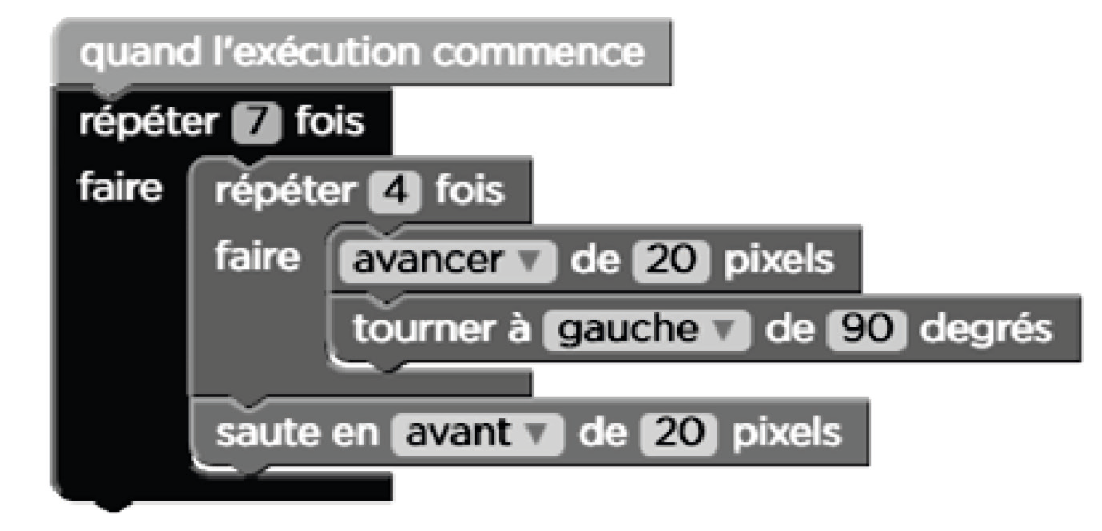
\includegraphics[width=8cm]{Transversal/Images/T15_ex_prog}
   \end{center}
   Quand il lance le programme, il obtient le {\it dessin 2}. \\
   Que faut-il modifier dans le programme pour obtenir le dessin attendu ?
   \begin{center}
      \begin{tabular}{cC{2.5}c}
         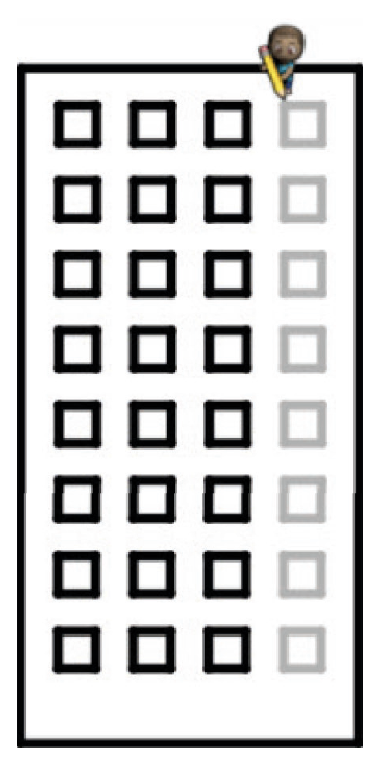
\includegraphics[width=2.2cm]{Transversal/Images/T15_ex_dessinf}
         &
         &
         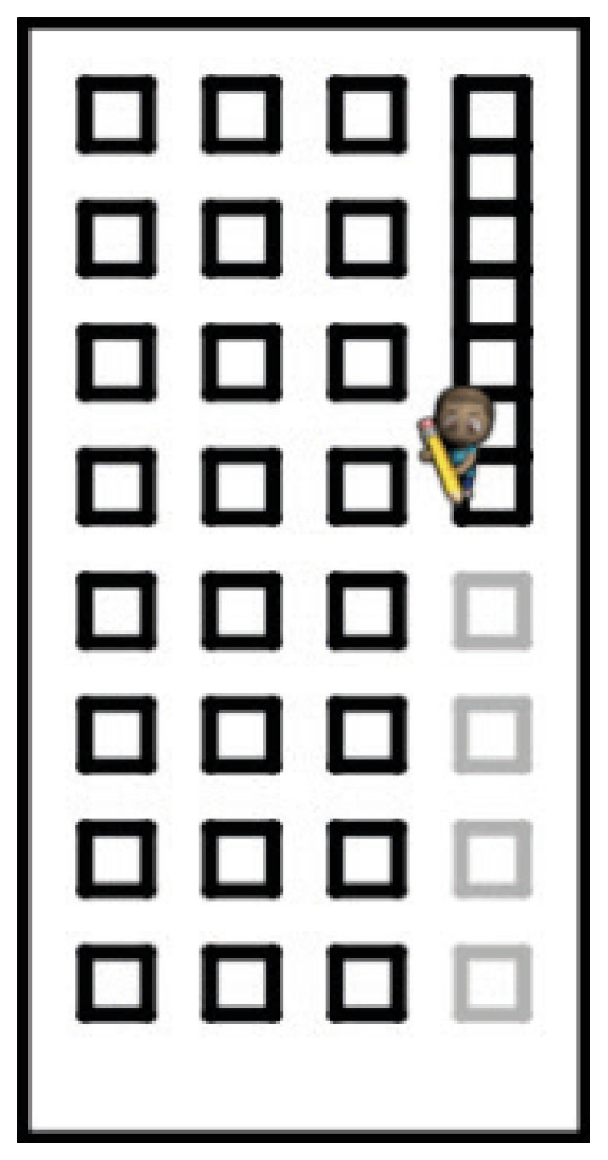
\includegraphics[width=2.2cm]{Transversal/Images/T15_ex_dessini} \\
         {\it dessin 1}
         &
         &
         {\it dessin 2} \\
      \end{tabular}
   \end{center}
\end{exercice}

\begin{corrige}
   On remarque que sur le dessin obtenu, les carrés ont été collés alors qu'il ont un décalage de 20 pixels sur le dessin d'origine. Ceci est dû au fait que le saut de 20 pixels est effectué au moment où le carré est terminé, lorsque le crayon se retrouve à sa position d'origine. Il faut donc effectuer un saut de 20 pixels pour arriver au sommet du carré, puis de 20 pixels pour laisser un espace, soit 40 pixels. \\
   De plus, il faut dessiner 8 carrés alors qu'il est indiqué de faire 7 répétitions. \\
   Conclusion : {\blue il faut remplacer 7 par 8 dans le bloc \og répéter 7 fois \fg{} et 20 par 40 dans le bloc \og Saute en avant de 20 pixels \fg}. \\
\end{corrige}

\bigskip



\begin{exercice}[CRPE 2017 G1]
   On utilise le programme ci-dessous.
   \begin{enumerate}
      \item Quel résultat s’affiche si l’on choisit d’entrer le nombre 7 ?
      \item Quel résultat s’affiche si l’on choisit d’entrer le nombre 12,7 ?
      \item Quel résultat s’affiche si l’on choisit d’entrer le nombre $-6$ ?
   \end{enumerate}
   \begin{center}
      \begin{scratch}    
         \blockinit{quand \greenflag est cliqué}
         \blocksensing{demander \ovalnum{Choisissez un nombre} et attendre}
         \blockifelse{si \booloperator{\ovalsensing{réponse} < \ovalnum{10}} alors}
            {\blockvariable{mettre \selectmenu{résultat} à \ovaloperator{\ovalnum{5} * \ovalsensing{réponse} + \ovalnum{3}}}}
            {\blockvariable{mettre \selectmenu{résultat} à \ovaloperator{\ovalnum{2} * \ovalsensing{réponse} - \ovalnum{7}}}}
         \blocklook{dire \ovaloperator{regroupe \ovalnum{Le nombre obtenu est} \ovalvariable{résultat}}}
      \end{scratch}
   \end{center}
\end{exercice}

\begin{corrige}
\ \\ [-5mm]
   \begin{enumerate}
      \item $7<10$ donc, le résultat vaut $5\times5+3 =$ {\blue 38}.
      \item $12,7\geq10$ donc, le résultat vaut $2\times12,7-7 =$ {\blue 18,4}.
      \item $-6<10$ donc, le résultat vaut $5\times(-6)+3=$ {\blue $-27$}.
   \end{enumerate}
\end{corrige}

\pagebreak


\begin{exercice}[CRPE 2017 G4]
   Voici un programme de calcul :
   \vspace*{-15mm}
   \begin{center}
      \begin{scratch}    
         \blockinit{quand \greenflag est cliqué}
         \blocksensing{demander \ovalnum{Donner une valeur} et attendre}
         \blockvariable{mettre \selectmenu{x} à \ovalsensing{réponse}}
         \blockvariable{mettre \selectmenu{A} à \ovaloperator{\ovalvariable{x} - \ovalnum{8}}}
         \blockvariable{mettre \selectmenu{B} à \ovaloperator{\ovalvariable{A} * \ovalnum{3}}} 
         \blockvariable{mettre \selectmenu{C} à \ovaloperator{\ovalvariable{B} + \ovalnum{24}}}
         \blockvariable{mettre \selectmenu{D} à \ovaloperator{\ovalvariable{C} + \ovalvariable{x}}}
         \blockvariable{montrer la variable \selectmenu{D}}
      \end{scratch}
   \end{center}
   \begin{enumerate}
      \item
         \begin{enumerate}
            \item On applique ce programme de calcul au nombre 10. Montrer que le résultat affiché à la fin est 40.
            \item On applique ce programme de calcul au nombre –2. Quel va être le résultat affiché à la fin ? Justifier.
         \end{enumerate}
      \item Une modification possible de l’algorithme est copiée ci-dessous, mais il manque une  instruction à la 4\up{ème} ligne.
         \begin{center}
            \begin{scratch}    
               \blockinit{quand \greenflag est cliqué}
               \blocksensing{demander \ovalnum{Donner une valeur} et attendre}
               \blockvariable{mettre \selectmenu{x} à \ovalsensing{réponse}}
               \blockvariable{mettre \selectmenu{A} à \ovalnum{}}
               \blockvariable{montrer la variable \selectmenu{A}}
            \end{scratch}
         \end{center} \medskip
         Comment compléter la 4\up{ème} ligne, là où il y a un carré blanc, par l’expression la plus simple possible pour que cet algorithme affiche le même résultat que l’algorithme précédent quel que soit le nombre entré ?
   \end{enumerate}
\end{exercice}

\begin{corrige}
\ \\ [-5mm]
\begin{enumerate}
   \item
   \begin{enumerate}
      \item En saisissant 10, on obtient successivement :
      \begin{itemize}
         \item $x =10$ ;
         \item A $= x-8 =10-8 =2$ ;
         \item B = A$\times3 =2\times3 =6$ ;
         \item C =  B $+24 =6+24 =30$ ;
         \item D = C $+x =30+10 =40$.
      \end{itemize}
      Donc, {\blue si le nombre choisi et 10, le résultat affiché est 40}.
      \item En saisissant $-2$, on obtient successivement :
      \begin{itemize}
         \item $x =-2$ ;
         \item A $= x-8 =-2-8 =-10$ ;
         \item B = A$\times3 =-10\times3 =-30$ ;
         \item C = B $+24 =-30+24 =-6$ ;
         \item D = C $+x =-6-2 =-8$.
      \end{itemize}
      Donc, {\blue si le nombre choisi et $-2$, le résultat affiché est $-8$}.
   \end{enumerate}
   \item On obtient successivement :
      \begin{itemize}
         \item $x$ ;
         \item A $= x-8$ ;
         \item B = A$\times3 =(x-8)\times3 =3x-24$ ;
         \item C = B $+24 =3x-24+24 =3x$ ;
         \item D = C $+x =3x+x =4x$.
      \end{itemize}
      Donc, {\blue il faut mettre l'expression $4x$ dans le carré blanc}.
\end{enumerate}
\end{corrige}

\bigskip


\begin{exercice}[CRPE 2017 G3]
   \begin{minipage}{8cm}
   Un élève utilise le programme ci-contre.
   \begin{enumerate}
      \item Quelle réponse le logiciel va-t-il afficher si l’élève entre la valeur 5 ? Expliquer pourquoi.
      \item Quel nombre l’élève doit-il rentrer pour obtenir en retour le message \og Bravo ! Tu as trouvé le nombre mystère. \fg ?
   \end{enumerate}
   \end{minipage}
   \hfill
   \begin{minipage}{8cm}
      \vspace*{-12mm}
      \begin{scratch}    
         \blockinit{quand \greenflag est cliqué}
         \blocksensing{demander \ovalnum{Quel est le nombre mystère ?} et attendre}
         \blockvariable{mettre \selectmenu{x} à \ovalsensing{réponse}}
         \blockifelse{si \booloperator{\ovaloperator{\ovaloperator{\ovalnum{3} * \ovalvariable{x}} + \ovalnum{7}} = \ovalnum{40}} alors}
            {\blocklook{dire \ovalnum{Bravo ! Tu as trouvé le nombre mystère}}}
            {\blocklook{dire \ovalnum{Et non désolée, ce n'est pas le nombre mystère}}}
      \end{scratch}
   \end{minipage}
\end{exercice}

\begin{corrige}
\ \\ [-5mm]
   \begin{enumerate}
      \item Si $x =5$, alors $3x+7 =3\times5+7 =22\neq40$ donc, le logiciel va afficher la réponse : {\blue Et non désolé, ce n'est pas le nombre mystère. Essaie encore !}
      \item Pour obtenir le message \og Bravo ! Tu as trouvé le nombre mystère. \fg, il faut déterminer $x$ tel que $3x+7 =40 \iff 3x =40-7$ \\
         \hspace*{17mm} $\iff 3x =33$ \\ [1mm]
         \hspace*{17mm} $\iff x =\dfrac{33}{3} =11$. \\ [1mm]
         {\blue Le nombre mystère est 11}.
   \end{enumerate}
\end{corrige}

\bigskip


\begin{exercice}[CRPE 2020 G4] %%%2
   \begin{enumerate}
      \item Voici un programme de calcul : \\
         \begin{center}
            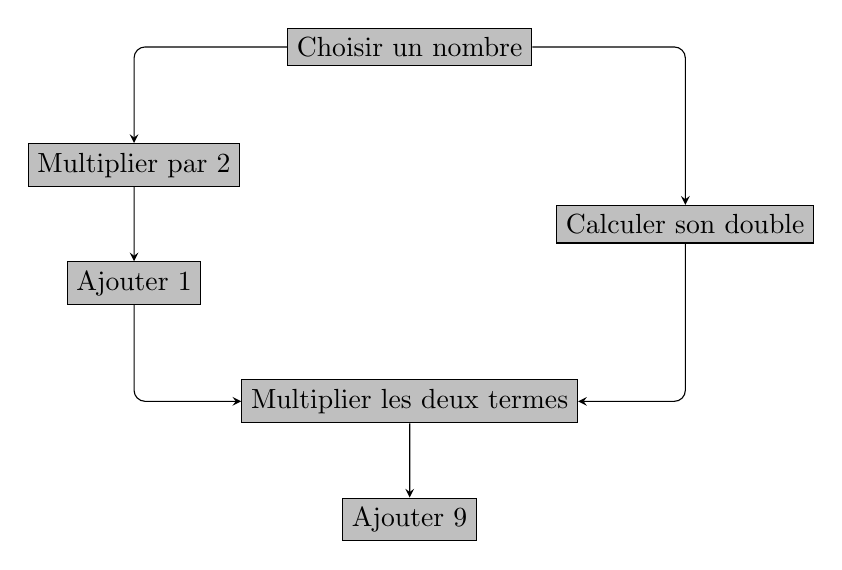
\begin{tikzpicture}[>=stealth,yscale=1.5,xscale=3.5]
               \node(choix) at (2,5)[rectangle,draw,fill=lightgray] {Choisir un nombre};
               \node(mul) at (1,4)[rectangle,draw,fill=lightgray] {Multiplier par 2};
               \node(aj) at (1,3)[rectangle,draw,fill=lightgray] {Ajouter 1}; 
               \node(cal) at (3,3.5)[rectangle,draw,fill=lightgray] {Calculer son double};     
               \node(mul2) at (2,2)[rectangle,draw,fill=lightgray] {Multiplier les deux termes};    
               \node(aj2) at (2,1)[rectangle,draw,fill=lightgray] {Ajouter 9};      
               \draw[->,rounded corners=4pt] (choix) -| (mul);
               \draw[->,rounded corners=4pt] (choix) -| (cal);
               \draw[->] (mul) -- (aj); 
               \draw[->,rounded corners=4pt] (aj) |- (mul2); 
               \draw[->,rounded corners=4pt] (cal) |- (mul2); 
               \draw[->] (mul2) -- (aj2); 
            \end{tikzpicture}
         \end{center}
         \begin{enumerate}
            \item Effectuer le programme de calcul en choisissant 2 comme nombre de départ et montrer qu’on obtient 29.
            \item Quel résultat obtient-on en choisissant $\dfrac23$ comme nombre de départ ? \smallskip
            \item Exprimer le résultat obtenu avec ce programme de calcul en prenant $x$ comme nombre de départ. \\ [-10mm]
         \end{enumerate}
      \item On teste un autre programme de calcul avec le logiciel Scratch :
         \begin{center}
            \begin{scratch}    
               \blockinit{quand \greenflag est cliqué}
               \blocksensing{demander \ovalnum{Choisir un nombre} et attendre}
               \blockvariable{mettre \selectmenu{résultat} à \ovaloperator{\ovalsensing{réponse} + \ovalnum{3}}}
               \blockvariable{mettre \selectmenu{résultat} à \ovaloperator{\ovalvariable{résultat} * \ovalvariable{résultat}}}
               \blocklook{dire \ovaloperator{regrouper \ovalnum{Le résultat est } et \ovalvariable{résultat}} pendant \ovalnum{2} secondes}
            \end{scratch}
         \end{center}
         \begin{enumerate}
            \item Effectuer le programme de calcul en choisissant 2 comme nombre de départ et montrer qu’on obtient 25.
            \item Quel résultat obtient-on en choisissant 1,5 comme nombre de départ ?
            \item Exprimer le résultat obtenu avec ce programme de calcul en prenant $x$ comme nombre de départ. \\ [-10mm]
         \end{enumerate}
      \item Déterminer pour quelle(s) valeur(s) de $x$ les deux programmes donnent le même résultat. Justifier la réponse.
   \end{enumerate}
\end{exercice}

\begin{corrige}
\ \\ [-5mm]
   \begin{enumerate}
      \item On obtient les organigrammes suivants : \vspace*{-3mm}
         \begin{multicols}{3}
            \begin{enumerate}
               \item Avec 2 : \\ [2mm]
                  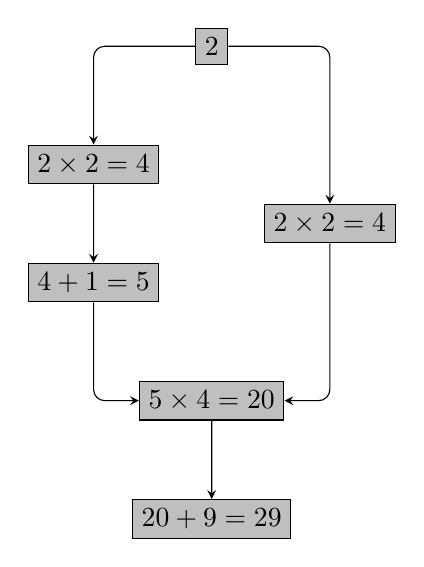
\begin{tikzpicture}[>=stealth,scale=1.5]
                     \node(choix) at (2,5)[rectangle,draw,fill=lightgray] {2};
                     \node(mul) at (1,4)[rectangle,draw,fill=lightgray] {$2\times2 =4$};
                     \node(aj) at (1,3)[rectangle,draw,fill=lightgray] {$4+1 =5$}; 
                     \node(cal) at (3,3.5)[rectangle,draw,fill=lightgray] {$2\times2 =4$};     
                     \node(mul2) at (2,2)[rectangle,draw,fill=lightgray] {$5\times4 =20$};
                     \node(aj2) at (2,1)[rectangle,draw,fill=lightgray] {$20+9 =29$};   
                     \draw[->,rounded corners=4pt] (choix) -| (mul);
                     \draw[->,rounded corners=4pt] (choix) -| (cal);
                     \draw[->] (mul) -- (aj); 
                     \draw[->,rounded corners=4pt] (cal) |- (mul2); 
                     \draw[->,rounded corners=4pt] (aj) |- (mul2); 
                    \draw[->] (mul2) -- (aj2); 
                  \end{tikzpicture} \\ [2mm]
                  {\blue Avec 2, on obtient 29}.
               \columnbreak
               \item Avec $\dfrac23$ : \\ [2mm]
                  \begin{tikzpicture}[>=stealth,scale=1.5]
                     \node(choix) at (2,5)[rectangle,draw,fill=lightgray] {$\dfrac23$};
                     \node(mul) at (1,4)[rectangle,draw,fill=lightgray] {$2\times\dfrac23 =\dfrac43$};
                     \node(aj) at (1,3)[rectangle,draw,fill=lightgray] {$\dfrac43+1 =\dfrac73$}; 
                     \node(cal) at (3,3.5)[rectangle,draw,fill=lightgray] {$2\times\dfrac23 =\dfrac43$};     
                     \node(mul2) at (2,2)[rectangle,draw,fill=lightgray] {$\dfrac73\times\dfrac43 =\dfrac{28}{9}$};
                     \node(aj2) at (2,1)[rectangle,draw,fill=lightgray] {$\dfrac{28}{9}+9 =\dfrac{109}{9}$};   
                     \draw[->,rounded corners=4pt] (choix) -| (mul);
                     \draw[->,rounded corners=4pt] (choix) -| (cal);
                     \draw[->] (mul) -- (aj); 
                     \draw[->,rounded corners=4pt] (cal) |- (mul2); 
                     \draw[->,rounded corners=4pt] (aj) |- (mul2); 
                    \draw[->] (mul2) -- (aj2); 
                  \end{tikzpicture} \\ [2mm]
                  {\blue Avec $\dfrac23$, on obtient $\dfrac{109}{9}$}.
               \columnbreak
               \item Avec $x$ : \\ [2mm]
                  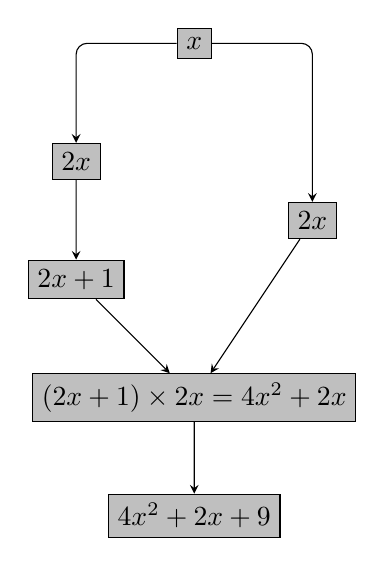
\begin{tikzpicture}[>=stealth,scale=1.5]
                     \node(choix) at (2,5)[rectangle,draw,fill=lightgray] {$x$};
                     \node(mul) at (1,4)[rectangle,draw,fill=lightgray] {$2x$};
                     \node(aj) at (1,3)[rectangle,draw,fill=lightgray] {$2x+1$}; 
                     \node(cal) at (3,3.5)[rectangle,draw,fill=lightgray] {$2x$};     
                     \node(mul2) at (2,2)[rectangle,draw,fill=lightgray] {$(2x+1)\times2x =4x^2+2x$};
                     \node(aj2) at (2,1)[rectangle,draw,fill=lightgray] {$4x^2+2x+9$};   
                     \draw[->,rounded corners=4pt] (choix) -| (mul);
                     \draw[->,rounded corners=4pt] (choix) -| (cal);
                     \draw[->] (mul) -- (aj); 
                     \draw[->,rounded corners=4pt] (cal) -- (mul2); 
                     \draw[->] (aj) -- (mul2); 
                    \draw[->] (mul2) -- (aj2); 
                  \end{tikzpicture} \\ [2mm]
                  {\blue Avec $x$, on obtient $4x^2+2x+9$}.   
            \end{enumerate}
         \end{multicols} 
      \setcounter{enumi}{1}
      \item On obtient les résultats suivants : \vspace*{-4mm}
         \begin{multicols}{3}
            \begin{enumerate}
               \item Avec 2 : \\
                  \begin{itemize}
                     \item réponse $\leftarrow$ 2
                     \item résultat $\leftarrow2+3 =5$
                     \item résultat $\leftarrow5\times5 =25$
                     \item {\blue \og le résultat est 25 \fg}.
                  \end{itemize}
                  \columnbreak
               \item Avec 1,5, on obtient : \\
                  \begin{itemize}
                     \item réponse $\leftarrow$ 1,5
                     \item résultat $\leftarrow1,5+3 =4,5$
                     \item résultat $\leftarrow4,5\times4,5 =20,25$
                     \item {\blue \og le résultat est 20,25 \fg}.
                  \end{itemize}
                  \columnbreak
               \item Avec $x$, on obtient : \\
                  \begin{itemize}
                     \item réponse $\leftarrow x$
                     \item résultat $\leftarrow x+3$
                     \item résultat $\leftarrow(x+3)\times(x+3) =x^2+6x+9$
                     \item {\blue \og le résultat est $x^2+6x+9$ \fg}.
                  \end{itemize}
                  \columnbreak
            \end{enumerate}
         \end{multicols}
      \setcounter{enumi}{2}
      \item $4x^2+2x+9 =x^2+6x+9 \iff 3x^2-4x =0$ \\ 
         \hspace*{4.3cm} $\iff x(3x-4)$ \\
         \hspace*{4.3cm} $\iff x =0 \text{ ou } 3x-4 =0$ \\ [1mm]
         \hspace*{4.3cm} $\iff x =0 \text{ ou } x=\dfrac43$ \\
         {\blue Les programmes donnent le même résultat pour des valeurs égales à 0 ou à $\dfrac43$}.
   \end{enumerate}
\end{corrige}

\newpage


\begin{exercice}[La fourmi de Langton]
   La fourmi de Langton, du nom de son inventeur scientifique américain {\it Christopher Langton}, est un petit programme informatique inventé vers la fin des années 1980. Il consiste en un automate qui se déplace dans un quadrillage suivant des règles suivantes :
      \begin{itemize}
         \item au départ, toutes les cases sont de la même couleur, ici blanches ;
         \item si la fourmi est sur une case blanche, elle tourne de \udeg{90} vers la droite, change la couleur de la case en noir et avance d'une case ;
         \item si la fourmi est sur une case noire, elle tourne de \udeg{90} vers la gauche, change la couleur de la case en blanc et avance d'une case.
      \end{itemize}
      Compléter dans les quadrillages ci-dessous les quinze premières étapes du déplacement de la fourni.
      \begin{center}
      \psset{unit=0.5,subgriddiv=1,gridlabels=0mm,gridcolor=gray,fillcolor=darkgray,fillstyle=solid}
      \small
         \begin{pspicture}(0,-0.7)(7,7)
            \psgrid(0,0)(7,7)
            \fourmi{3.5}{3.5}{0}
            \rput(3.5,-0.5){étape 0}
         \end{pspicture}
         \quad
         \begin{pspicture}(0,-0.7)(7,7)
            \psframe(3,3)(4,4)
            \psgrid(0,0)(7,7)
            \fourmi{4.5}{3.5}{-90}
            \rput(3.5,-0.5){étape 1}
         \end{pspicture}
         \quad
         \begin{pspicture}(0,-0.7)(7,7)  
            \psframe(3,3)(5,4)
            \psgrid(0,0)(7,7)
            \fourmi{4.5}{2.5}{180}
            \rput(3.5,-0.5){étape 2}
         \end{pspicture}
         \quad
         \begin{pspicture}(0,-0.7)(7,7)
            \psgrid(0,0)(7,7)
            \rput(3.5,-0.5){étape 3}
         \end{pspicture}
         \bigskip
         \begin{pspicture}(0,-0.7)(7,7)
            \psframe(3,2)(5,4)
            \psgrid(0,0)(7,7)
            \fourmi{3.5}{3.5}{0}
            \rput(3.5,-0.5){étape 4}
         \end{pspicture}
         \quad
         \begin{pspicture}(0,-0.7)(7,7)
            \psgrid(0,0)(7,7)
            \rput(3.5,-0.5){étape 5}
         \end{pspicture}
         \quad
         \begin{pspicture}(0,-0.7)(7,7)
            \psgrid(0,0)(7,7)
            \rput(3.5,-0.5){étape 6}
         \end{pspicture}
         \quad
         \begin{pspicture}(0,-0.7)(7,7)
            \psframe(2,3)(3,5)
            \pspolygon(3,2)(5,2)(5,4)(4,4)(4,3)(3,3)
            \psgrid(0,0)(7,7)
            \fourmi{3.5}{4.5}{-90}
            \rput(3.5,-0.5){étape 7}
         \end{pspicture}
         \bigskip
         \begin{pspicture}(0,-0.7)(7,7)
            \psgrid(0,0)(7,7)
            \rput(3.5,-0.5){étape 8}
         \end{pspicture}
         \quad
         \begin{pspicture}(0,-0.7)(7,7)
            \psgrid(0,0)(7,7)
            \rput(3.5,-0.5){étape 9}
         \end{pspicture}
         \quad
         \begin{pspicture}(0,-0.7)(7,7)
            \psgrid(0,0)(7,7)
            \rput(3.5,-0.5){étape 10}
         \end{pspicture}
         \quad
         \begin{pspicture}(0,-0.7)(7,7)
            \pspolygon(2,2)(5,2)(5,4)(4,4)(4,5)(2,5)(2,4)(3,4)(3,3)(2,3)
            \psgrid(0,0)(7,7)
            \rput(3.5,-0.5){étape 11}
            \fourmi{1.5}{2.5}{90}
         \end{pspicture}
         \bigskip
         \begin{pspicture}(0,0)(7,7)
         \psgrid(0,0)(7,7)
            \rput(3.5,-0.5){étape 12}
         \end{pspicture}
         \quad
         \begin{pspicture}(0,0)(7,7)
            \psgrid(0,0)(7,7)
            \rput(3.5,-0.5){étape 13}
         \end{pspicture}
         \quad
         \begin{pspicture}(0,0)(7,7)
            \psgrid(0,0)(7,7)
            \rput(3.5,-0.5){étape 14}
         \end{pspicture}
         \quad
         \begin{pspicture}(0,0)(7,7)
            \psgrid(0,0)(7,7)
            \rput(3.5,-0.5){étape 15}
         \end{pspicture} 
   \end{center}
   Ce programme modélise le fait qu'un ensemble de comportements élémentaires peut donner lieu à un comportement complexe. Pour voir ce qu'il se passe ensuite : \href{https://www.youtube.com/watch?v=qZRYGxF6D3w}{\it La fourmi de Langton, chaîne YouTube Science étonnante}.
\end{exercice}

\begin{corrige}
On obtient les quinze étapes suivantes :
   \begin{center}
      \psset{unit=0.5,subgriddiv=1,gridlabels=0mm,gridcolor=gray,fillstyle=solid,fillcolor=darkgray}
      \small
         \begin{pspicture}(0,-1.5)(7,7)
            \psgrid(0,0)(7,7)
            \fourmi{3.5}{3.5}{0}
            \rput(3.5,-0.5){étape 0}
         \end{pspicture}
         \quad
         \begin{pspicture}(0,-1.5)(7,7)
            \psframe(3,3)(4,4)
            \psgrid(0,0)(7,7)
            \fourmi{4.5}{3.5}{-90}
            \rput(3.5,-0.5){étape 1}
         \end{pspicture}
         \quad
         \begin{pspicture}(0,-1.5)(7,7)  
            \psframe(3,3)(5,4)
            \psgrid(0,0)(7,7)
            \fourmi{4.5}{2.5}{180}
            \rput(3.5,-0.5){étape 2}
         \end{pspicture}
         \quad
         \begin{pspicture}(0,-1.5)(7,7)
            \psframe[fillcolor=blue](3,3)(5,4)
            \psframe[fillcolor=blue](4,2)(5,3)
            \fourmi{3.5}{2.5}{90}
            \psgrid(0,0)(7,7)
            \rput(3.5,-0.5){étape 3}
         \end{pspicture}
         \bigskip
         \begin{pspicture}(0,-0.7)(7,7)
            \psframe(3,2)(5,4)
            \psgrid(0,0)(7,7)
            \fourmi{3.5}{3.5}{0}
            \rput(3.5,-0.5){étape 4}
         \end{pspicture}
         \quad
         \begin{pspicture}(0,-0.7)(7,7)
            \pspolygon[fillcolor=blue](3,2)(5,2)(5,4)(4,4)(4,3)(3,3)
            \fourmi{2.5}{3.5}{90}
            \psgrid(0,0)(7,7)
            \rput(3.5,-0.5){étape 5}
         \end{pspicture}
         \quad
         \begin{pspicture}(0,-0.7)(7,7)
            \pspolygon[fillcolor=blue](3,2)(5,2)(5,4)(4,4)(4,3)(3,3)
            \psframe[fillcolor=blue](2,3)(3,4)
            \fourmi{2.5}{4.5}{0}
            \psgrid(0,0)(7,7)
            \rput(3.5,-0.5){étape 6}
         \end{pspicture}
         \quad
         \begin{pspicture}(0,-0.7)(7,7)
            \psframe(2,3)(3,5)
            \pspolygon(3,2)(5,2)(5,4)(4,4)(4,3)(3,3)
            \psgrid(0,0)(7,7)
            \fourmi{3.5}{4.5}{-90}
            \rput(3.5,-0.5){étape 7}
         \end{pspicture}
         \bigskip
         \begin{pspicture}(0,-0.7)(7,7)
            \psframe(2,3)(3,5)
            \pspolygon(3,2)(5,2)(5,4)(4,4)(4,3)(3,3)
            \psframe(3,4)(4,5)
            \fourmi{3.5}{3.5}{180}
            \psgrid(0,0)(7,7)
            \rput(3.5,-0.5){étape 8}
         \end{pspicture}
         \quad
         \begin{pspicture}(0,-0.7)(7,7)
            \pspolygon[fillcolor=blue](3,2)(5,2)(5,4)(4,4)(4,5)(2,5)(2,3)(3,3)
            \fourmi{2.5}{3.5}{90}
            \psgrid(0,0)(7,7)
            \rput(3.5,-0.5){étape 9}
         \end{pspicture}
         \quad
         \begin{pspicture}(0,-0.7)(7,7)
            \pspolygon[fillcolor=blue](3,2)(5,2)(5,4)(4,4)(4,5)(2,5)(2,4)(3,4)
            \fourmi{2.5}{2.5}{180}
            \psgrid(0,0)(7,7)
            \rput(3.5,-0.5){étape 10}
         \end{pspicture}
         \quad
         \begin{pspicture}(0,-0.7)(7,7)
            \pspolygon(2,2)(5,2)(5,4)(4,4)(4,5)(2,5)(2,4)(3,4)(3,3)(2,3)
            \psgrid(0,0)(7,7)
            \rput(3.5,-0.5){étape 11}
            \fourmi{1.5}{2.5}{90}
         \end{pspicture}
         \bigskip
         \begin{pspicture}(0,-1)(7,7)
            \pspolygon[fillcolor=blue](1,2)(5,2)(5,4)(4,4)(4,5)(2,5)(2,4)(3,4)(3,3)(1,3)
            \fourmi{1.5}{3.5}{0}
            \psgrid(0,0)(7,7)
            \rput(3.5,-0.5){étape 12}
         \end{pspicture}
         \quad
         \begin{pspicture}(0,-1)(7,7)
            \pspolygon[fillcolor=blue](1,2)(5,2)(5,4)(4,4)(4,5)(2,5)(2,4)(3,4)(3,3)(2,3)(2,4)(1,4)
            \fourmi{2.5}{3.5}{-90}
            \psgrid(0,0)(7,7)
            \rput(3.5,-0.5){étape 13}
         \end{pspicture}
         \quad
         \begin{pspicture}(0,-1)(7,7)
            \pspolygon[fillcolor=blue](1,2)(5,2)(5,4)(4,4)(4,5)(2,5)(2,4)(1,4)
            \fourmi{2.5}{2.5}{180}
            \psgrid(0,0)(7,7)
            \rput(3.5,-0.5){étape 14}
         \end{pspicture}
         \quad
         \begin{pspicture}(0,-1)(7,7)
            \pspolygon[fillcolor=blue](1,2)(2,2)(2,3)(3,3)(3,2)(5,2)(5,4)(4,4)(4,5)(2,5)(2,4)(1,4)
            \fourmi{3.5}{2.5}{-90}
            \psgrid(0,0)(7,7)
            \rput(3.5,-0.5){étape 15}
         \end{pspicture} 
   \end{center}
\end{corrige}


